\section{Reflected row wrapping}\label[section]{sec:realization}

We prove \Cref{thm:r}. On a phase $[a,b]$ of positive length put $h=(b-a)/2$ and give job $j$ a first-half length $\ell_j=hz_j$. Place the job segments consecutively in index order on a line, then partition the line into rows of length $h$. Each row corresponds to a machine, with the position within the row giving the operation time in $[0,h)$. Empty pieces are discarded. The total length is at most $mh$ and at most $nh$, so at most $\min(m,n)$ rows are occupied. Every job has length at most $h$. It can meet at most two rows in positive length.

Row intervals are disjoint on each machine. If a job wraps, starting at local time $s$ in one row, its two operations occupy $[s,h)$ and $[0,r)$, with $r=\ell_j-(h-s)\leq s$. So the job is not processed on two machines at the same time. The same conclusion holds if $r=s$, with half-open endpoints. Translate the first-half operations by $a$. For each operation $[s,e)$ in absolute time add its reflection $[a+b-e,a+b-s)$ on the same machine for the same job. Reflection reverses order and preserves nonoverlap within the other half. The two halves are disjoint as half-open intervals. \Cref{fig:reflection} shows a wrapped job and its reflected operations.

Each job has total work $2\ell_j=(b-a)z_j$. The indicator satisfies $\sigma_j(a+b-t)=\sigma_j(t)$ almost everywhere. The change of variable $t\mapsto a+b-t$ gives, for its first moment $I_j$ on this phase,
\[
 I_j=(a+b)\int_a^b\sigma_j(t)\dt-I_j.
\]
Substituting the workload proves \eqref{eq:target-moments}. This holds for any rational shift, since the integrals on the bounded interval exist also for signed $t$. The case $a=b$ has zero work and first moment and requires no records. Consecutive phases meet only at excluded right endpoints, so their machine and job assignments can be concatenated. These arguments also cover zero rates, exact row fills and idle machines.

The row pieces of a job have endpoints computed by sums of the half-lengths and subtractions of row boundaries. One can scan the jobs in order maintaining the current occupied row and position, splitting only across the next boundary if necessary. This uses at most two first-half pieces per job and then copies their reflections. Hence there are at most $4nq$ nonempty records. Sorting their endpoints gives $O(nq)$ global event intervals (including gaps), with at most $n$ active assignments each. Products, sums over at most $n$ rational lengths per phase, comparisons and reflection have polynomial encoding and bit time by the arithmetic rules in \Cref{app:encoding}. This is the constructive proof of \Cref{thm:r}.

\begin{figure}[tbp]
\centering
\begin{tikzpicture}[x=2.32cm,y=0.63cm,font=\small]
 \node[anchor=west] at (0,9.05) {(a) Constant fractional rates};
 
 \foreach \y/\rate/\job/\shade in {8.25/{3/4}/1/14,7.59/{1/2}/2/35,6.93/{1/2}/3/6}{
   \draw[fill=black!\shade] (0,\y) rectangle (2,{\y+.18});
   \node[anchor=west,inner sep=2pt] at (2,{\y+.09}) {$z_\job=\rate$};
 }
 \node[below,inner sep=1pt] at (0,6.79) {$0$};
 \node[below,inner sep=1pt] at (2,6.79) {$2$};
 \node[anchor=west] at (0,5.9) {(b) Row wrapping on the first half};
 \foreach \y/\mach in {4.95/1,4.22/2}{
   \draw (0,\y) rectangle (1,{\y+.48});
   \node[anchor=east] at (0,{\y+.24}) {$M_{\mach}$};
 }
 \draw[fill=black!14] (0,4.95) rectangle node {$1$} (.75,5.43);
 \draw[fill=black!35] (.75,4.95) rectangle node {$2$} (1,5.43);
 \draw[fill=black!35] (0,4.22) rectangle node {$2$} (.25,4.70);
 \draw[fill=black!6] (.25,4.22) rectangle node {$3$} (.75,4.70);
 \foreach \x/\labeltext in {0/0,.25/{\tfrac14},.75/{\tfrac34},1/1}{
   \draw (\x,4.08) -- (\x,3.94);
   \node[below] at (\x,3.94) {$\labeltext$};
 }
 \draw (0,4.01) -- (1,4.01);
 \node[anchor=west] at (0,2.84) {(c) First half and its reflection};
 \foreach \y/\mach in {1.95/1,1.22/2}{
  \draw (0,\y) rectangle (2,{\y+.48});
  \node[anchor=east] at (0,{\y+.24}) {$M_{\mach}$};
 }
 \draw[fill=black!14] (0,1.95) rectangle node {$1$} (.75,2.43);
 \draw[fill=black!35] (.75,1.95) rectangle node {$2$} (1,2.43);
 \draw[fill=black!35] (1,1.95) rectangle node {$2$} (1.25,2.43);
 \draw[fill=black!14] (1.25,1.95) rectangle node {$1$} (2,2.43);
 \draw[fill=black!35] (0,1.22) rectangle node {$2$} (.25,1.70);
 \draw[fill=black!6] (.25,1.22) rectangle node {$3$} (.75,1.70);
 \draw[fill=black!6] (1.25,1.22) rectangle node {$3$} (1.75,1.70);
 \draw[fill=black!35] (1.75,1.22) rectangle node {$2$} (2,1.70);
 \draw[densely dashed] (1,2.57) -- (1,1.10);
 \draw (0,1.01) -- (2,1.01);
 \foreach \x/\labeltext in {0/0,.25/{\tfrac14},.75/{\tfrac34},1/1,1.25/{\tfrac54},1.75/{\tfrac74},2/2}{
   \draw (\x,1.08) -- (\x,.94);
   \node[below] at (\x,.94) {$\labeltext$};
 }
\end{tikzpicture}
\caption{Reflected realization on two machines. The cells are labeled by job and blank cells are idle. Job~2 wraps between the two rows in the first half. Reflection about time~1 keeps each operation on its assigned machine.}\label[figure]{fig:reflection}
\end{figure}


Ordinary wrapping over the full interval can change individual moments. For $[0,1]$, one machine and rates $(1/2,1/2)$, both fractional first moments are $1/4$. Serving job 1 on $[0,1/2)$ followed by job 2 on $[1/2,1)$ gives first moments $(1/8,3/8)$. With coefficients $(1,2)$ the fractional cost is $3/4$, compared with $7/8$ for that order and $5/8$ for its reverse. Reflection makes each job's first moment equal to its workload times the phase midpoint.
